\documentclass[a4paper, 11pt]{article}
\usepackage[top=3cm, bottom=3cm, left=3cm, right=3cm]{geometry}
\usepackage[utf8]{inputenc}
\usepackage[spanish, es-tabla]{babel}
\setlength{\parskip}{1em}
\usepackage{amsmath}
\usepackage{graphicx}
\usepackage{hyperref}

\usepackage{listings}
\usepackage{color}

\definecolor{mygreen}{rgb}{0,0.6,0}
\definecolor{mygray}{rgb}{0.5,0.5,0.5}
\definecolor{mymauve}{rgb}{0.58,0,0.82}

\lstset{
	backgroundcolor=\color{white},
	breaklines=true,
	commentstyle=\color{mygreen},
	keywordstyle=\color{blue},
	numberstyle=\tiny\color{mygray},
	stringstyle=\color{mymauve},
	tabsize=2
}

\usepackage{etoolbox}
\appto\appendix{\addtocontents{toc}{\protect\setcounter{tocdepth}{0}}}
\appto\listoffigures{\addtocontents{lof}{\protect\setcounter{tocdepth}{1}}}
\appto\listoftables{\addtocontents{lot}{\protect\setcounter{tocdepth}{1}}}

\begin{document}
\pagenumbering{gobble}
\begin{titlepage}
	\centering
	
\includegraphics[width=0.25\textwidth]{fib.png}\par
	\vspace{2cm}
	{\scshape\LARGE Facultat Informàtica de Barcelona \par}
	\vspace{1cm}
	{\scshape\Large Internet of Things\par}
	\vspace{1cm}
	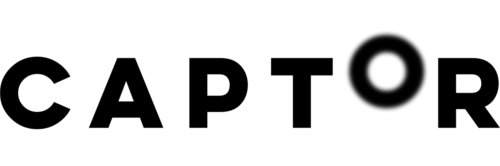
\includegraphics[width=0.5\textwidth]{../logo.png}\par
	\vspace{0.5cm}
	{\huge\bfseries Informe\par}
	\vspace{0.5cm}
	{\Large\itshape Conexionado de anemómetro y veleta\par}
	\vspace{2cm}
	{\large \today\par}
\end{titlepage}
\newpage

\pagenumbering{arabic}
\tableofcontents
\newpage

\listoffigures
\listoftables
\newpage

\section{Introducción}
Actualmente, la contaminación del aire es controlada por redes de estaciones equipadas con instrumentos de referencia de alta calidad. como consecuencia del elevado coste, las estaciones cubren una densidad espacial relativamente baja, que se transforma en una reproducción poco precisa de la variabilidad de las concentraciones. Debido al avance en sensores móviles y aplicaciones de software, ha surgido un creciente  interés en redes de sensores basados en los ciudadanos.

El \textbf{Proyecto Captor}\footnote{\url{https://www.captor-project.eu/es/}} es un proyecto desarrollado por la \texttt{Universitat Politècnica de Catalunya} juntamente con la \texttt{Université Blaise Pascal Clermont-Ferrand} y otras organizaciones. El objetivo es establecer redes de sensores de bajo coste mantenidos por los ciudadanos para medir la contaminación de ozono en áreas dispersas.

Los datos del proyecto se recogerán entre el día 01/01/2015 y 31/12/2017 en 3 zonas europeas muy afectadas por la contaminación de ozono:

\begin{itemize}
	\item Barcelonès - Vallès Occidental - Osona (Cataluña, España)
	\item Pianura Padana (Calle del Po, Itàlia)
	\item Burgenland, Steiermark and Niederösterreich (Austria)
\end{itemize}

El dispositivo encargado de capturar los datos se muestra en la figura \ref{fig:captor}. La finalidad de este trabajo es ampliar los captor para que puedan capturar información sobre el viento.

\begin{figure}[h]
\centering
	\begin{minipage}{0.5\textwidth}
	\centering
	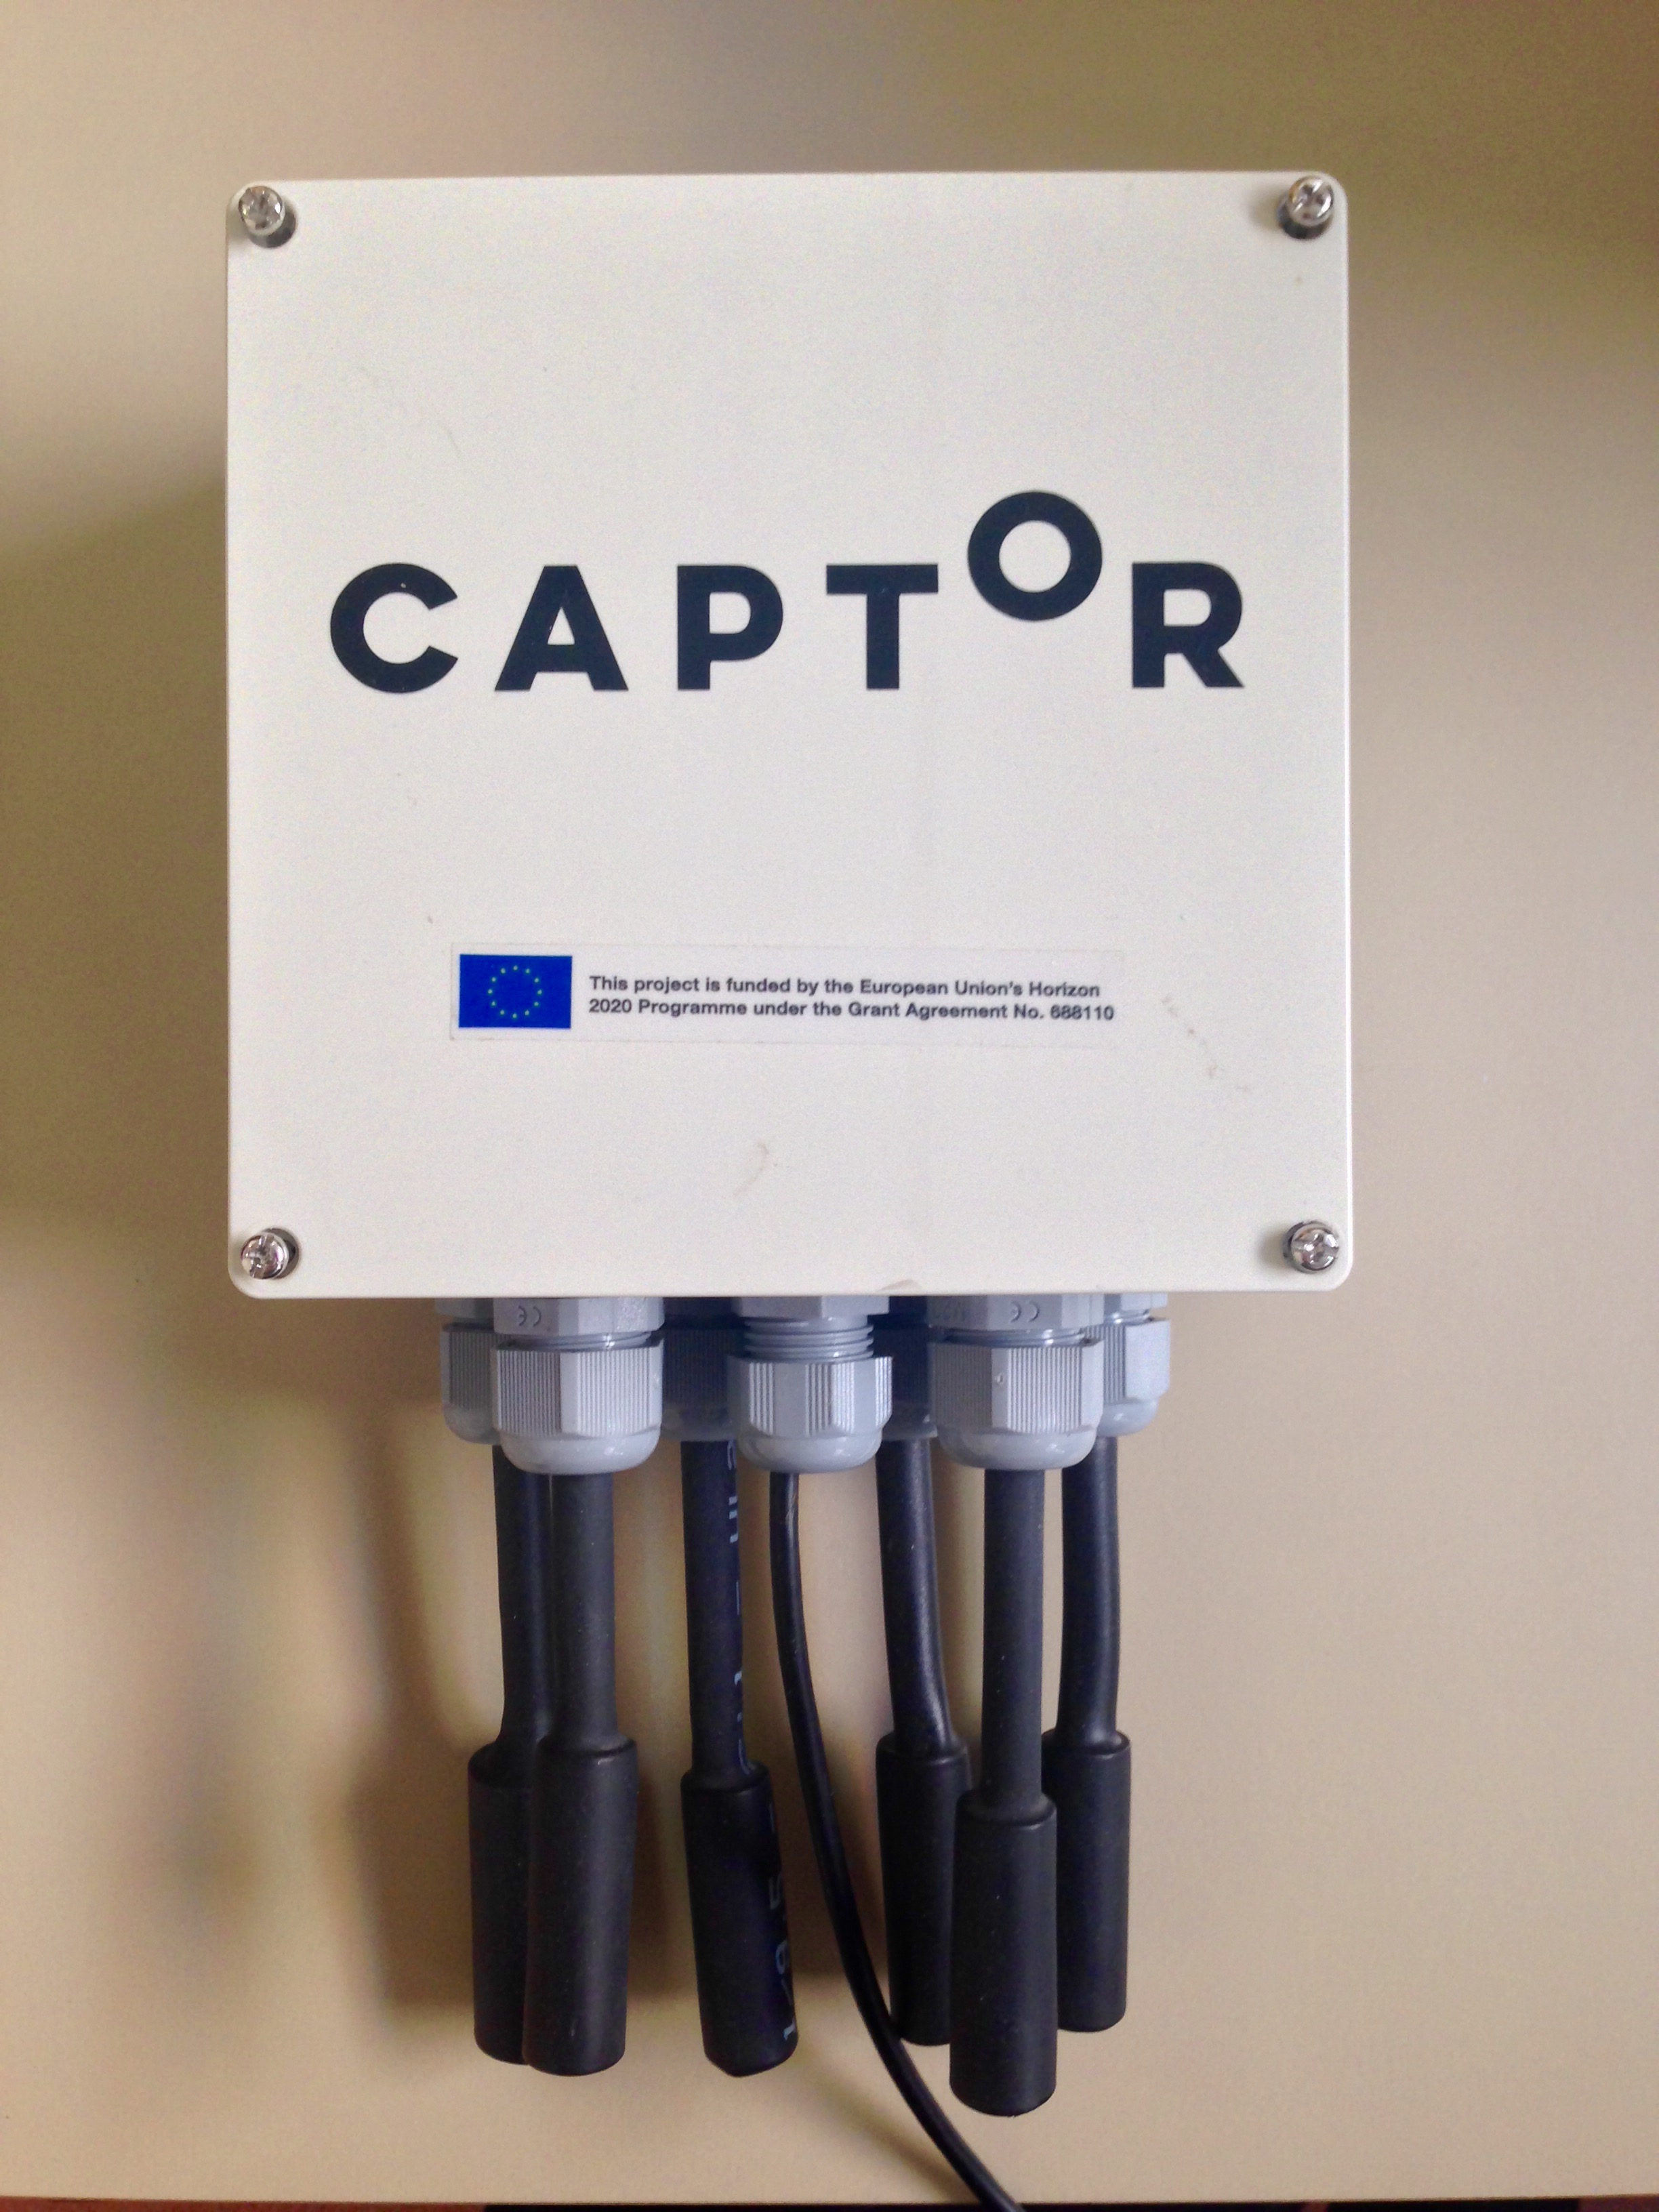
\includegraphics[width=0.75\textwidth]{img/Captor1.jpg}
	\end{minipage}%
	\begin{minipage}{0.5\textwidth}
	\centering
	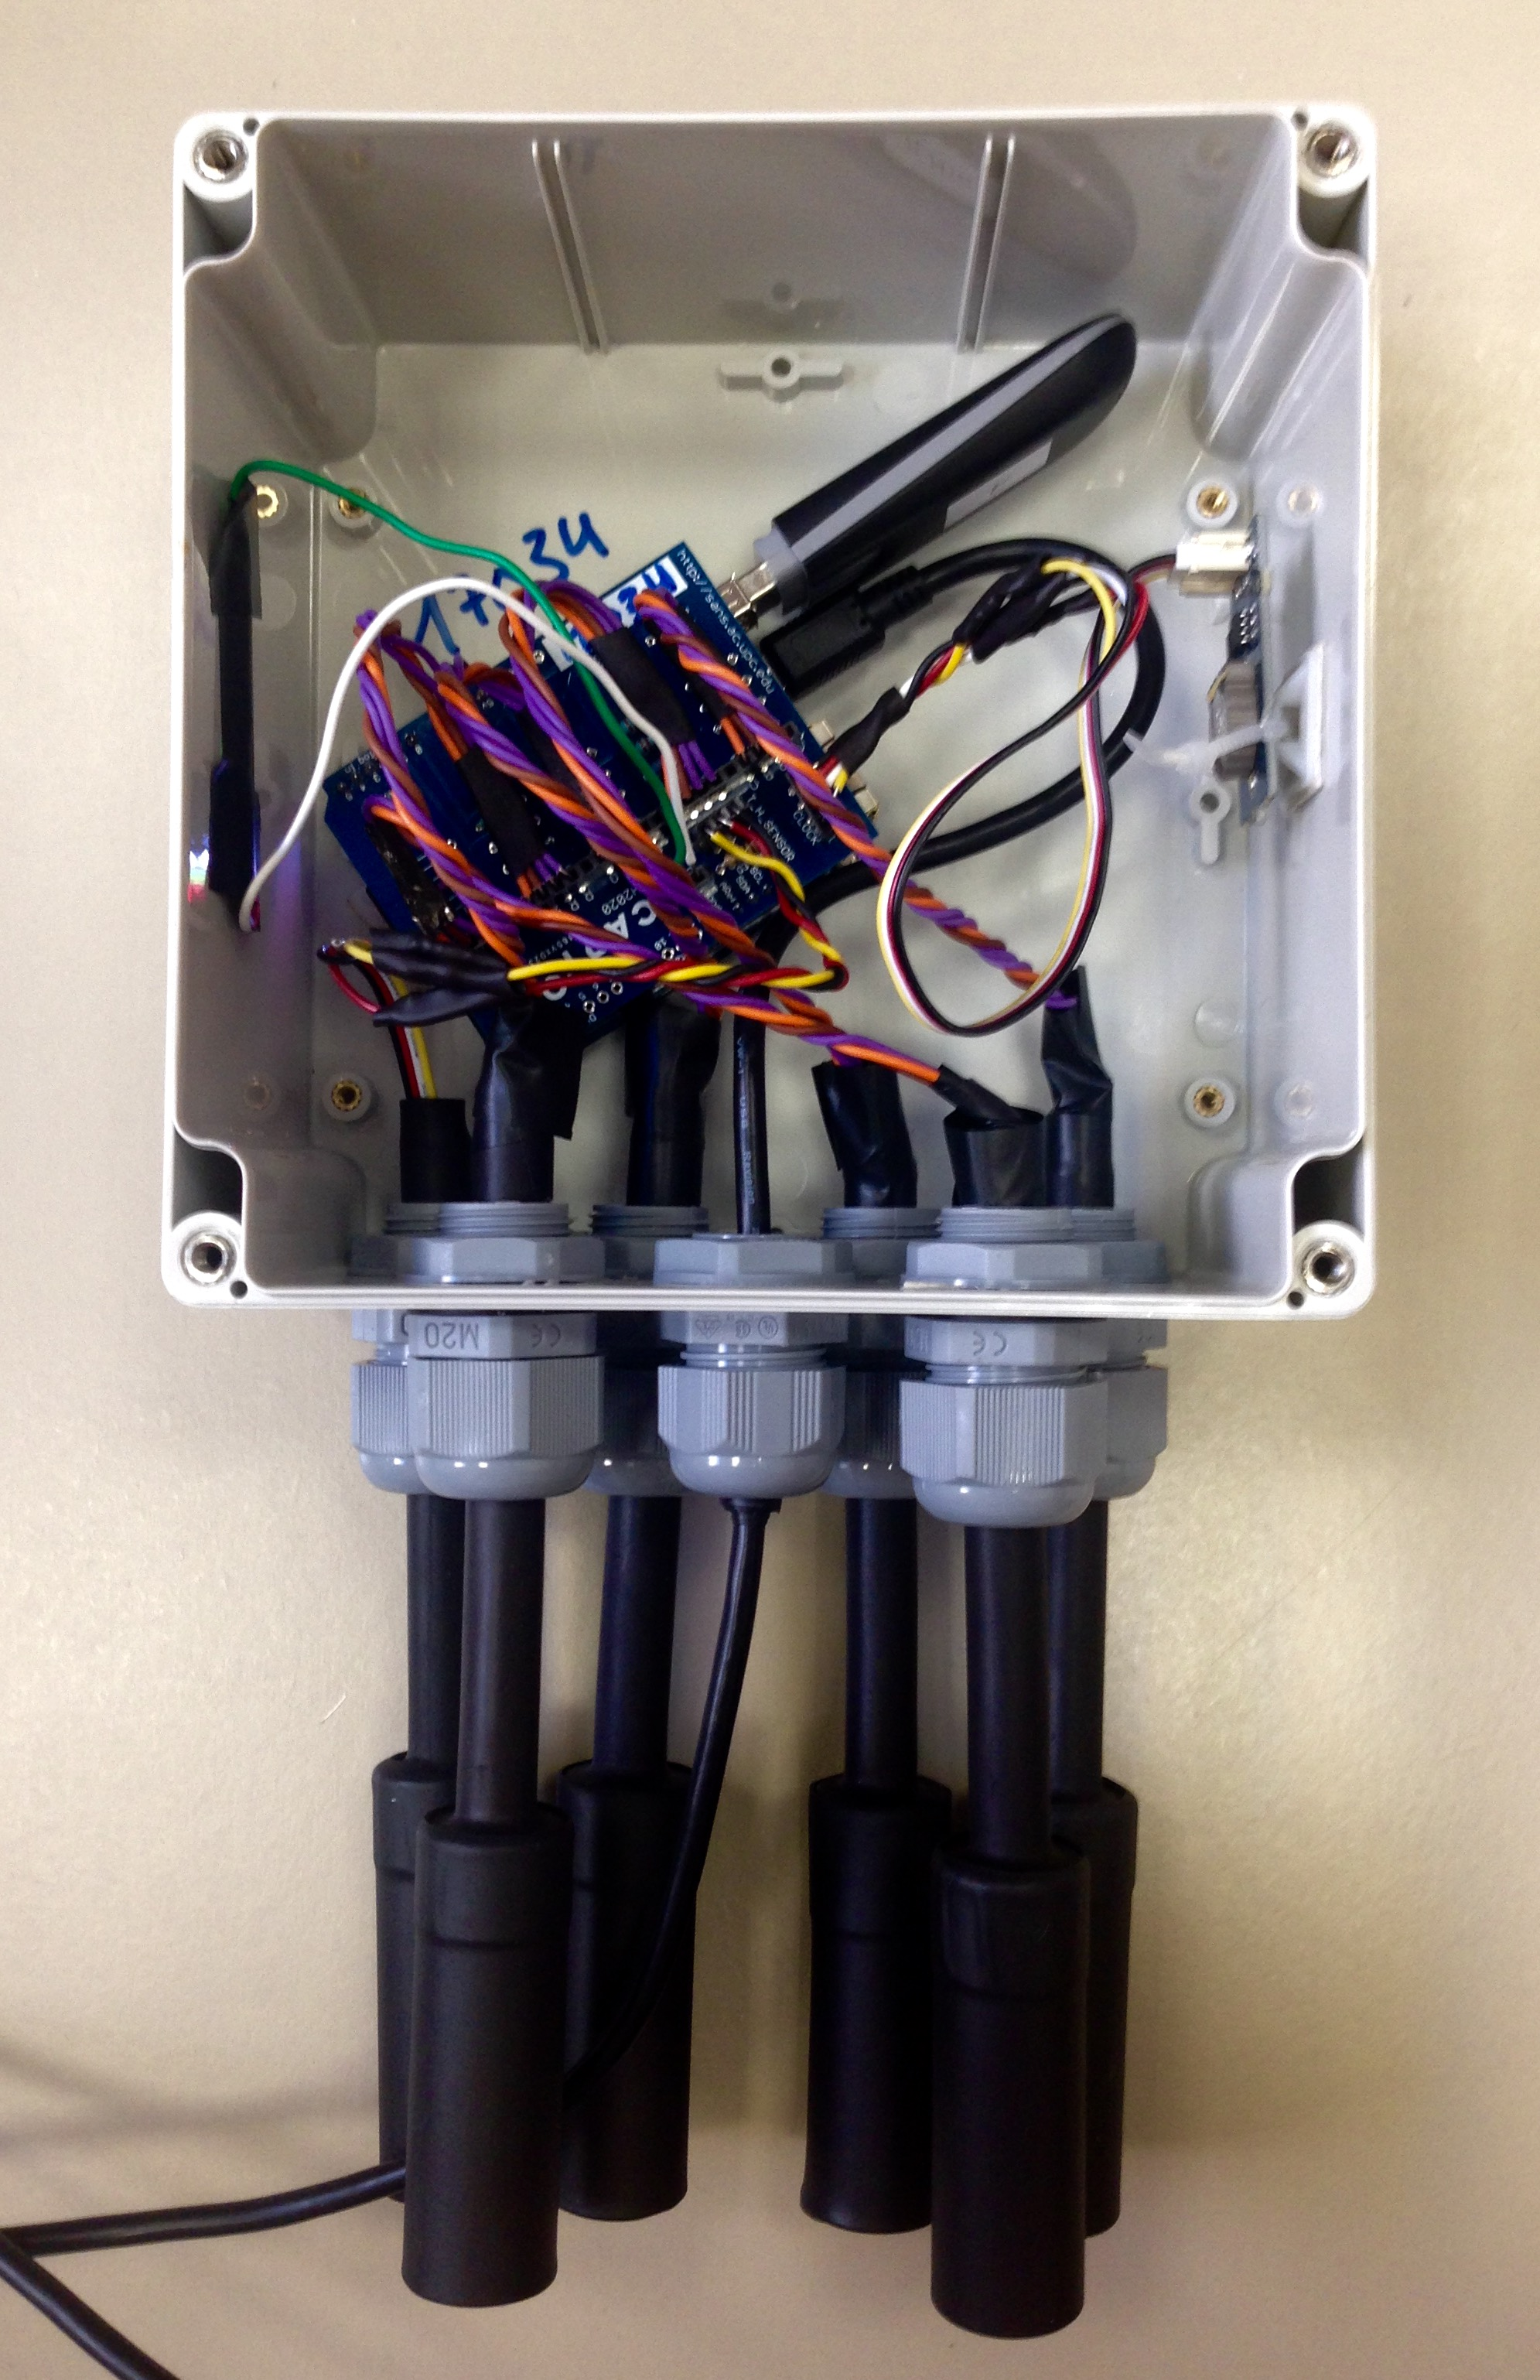
\includegraphics[width=0.75\textwidth]{img/Captor2.jpg}
	\end{minipage}
\caption{Dispositivo captor}
\label{fig:captor}
\end{figure}
\newpage

\section{El viento}
Porqué añadimos sensores para monitorizar el viento?
Que datos extraemos?
Que relación tienen los datos del viento con el ozono?
\newpage

\section{El dispositivo}
Para obtener datos sobre la velocidad y dirección del viento se usa anemómetro y veleta de la marca Davis\footnote{\url{http://www.davisnet.com/product/anemometer-for-weather-monitor-or-wizard/}} (figura \ref{fig:gadget}). El sensor de velocidad del viento usa un interruptor magnético que se activa por cada revolución de las aspas. La dirección del viento es mesurada a través de un potenciómetro.

\begin{figure}[h]
	\center
	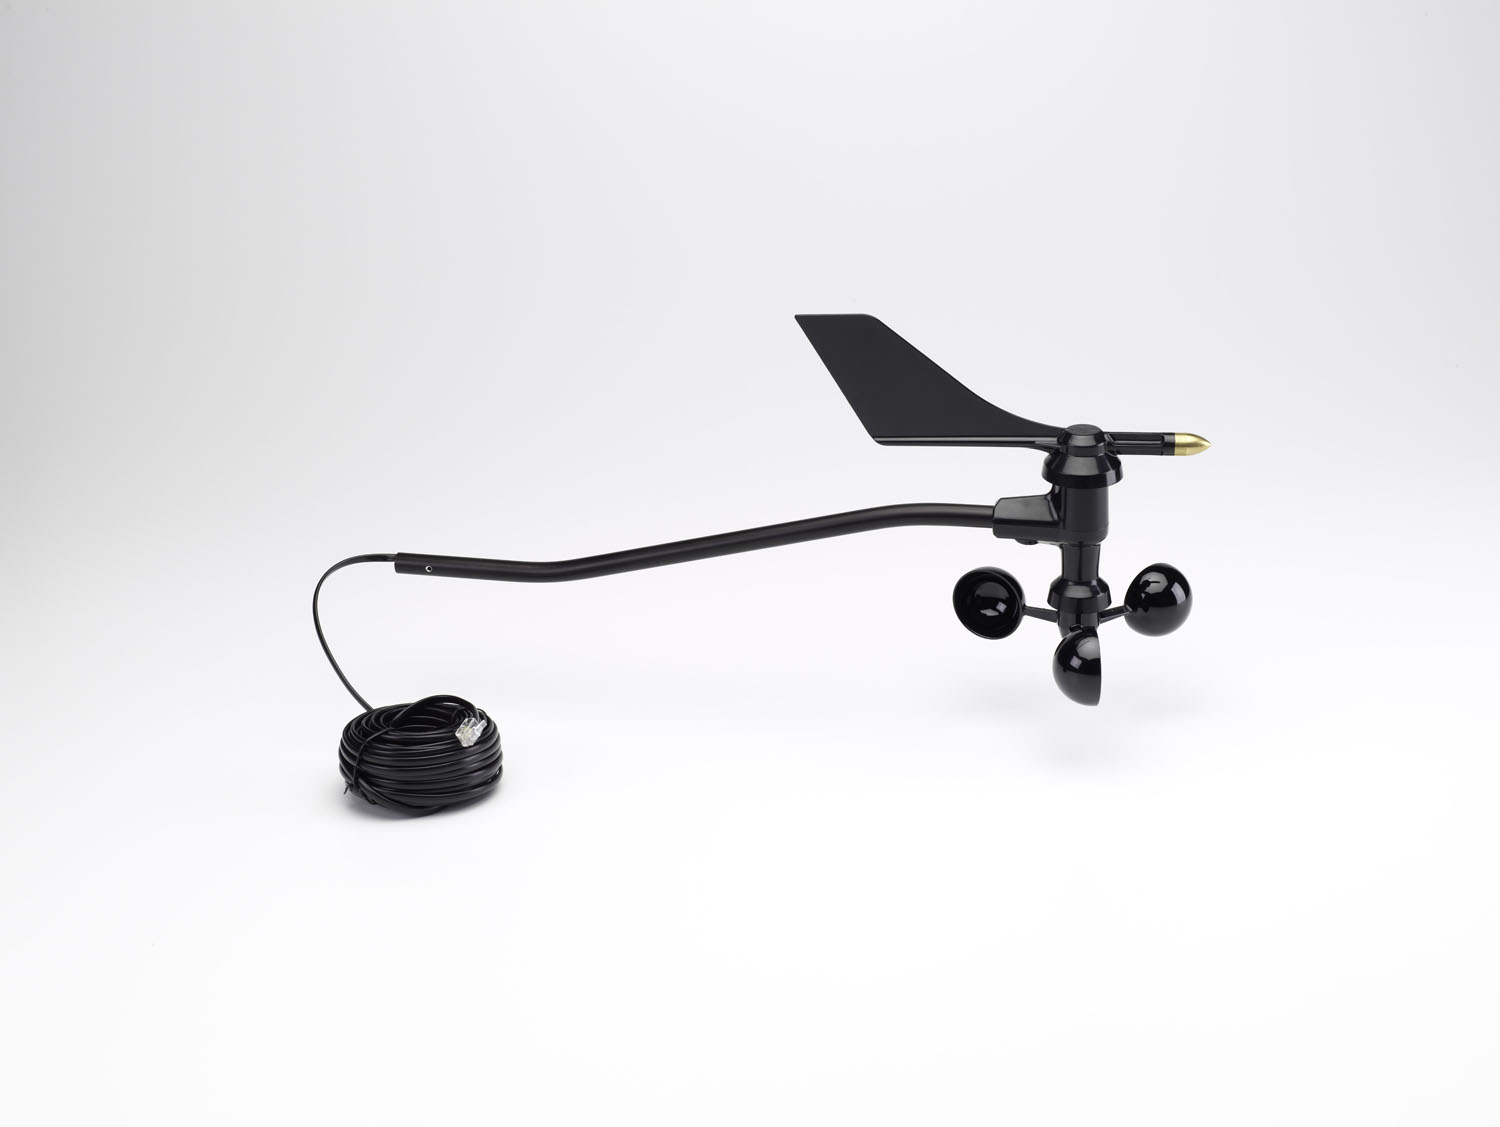
\includegraphics[width=0.65\textwidth]{img/davis.jpg}
	\caption{Dispositivo}
	\label{fig:gadget}
\end{figure}

Algunas de las especificaciones más relevantes que presenta el dispositivos se describen a la tabla 	\ref{tab:specifications}.

\begin{table}[h]
\center
\begin{tabular}{| c | c | c |}
\hline
& \textbf{Velocidad} & \textbf{Dirección} \\
\hline
Rango & 1 - 322 km/h & 0 - 360º \\
\hline
Precisión & $\pm$3 km/h & $\pm$7º \\
\hline
Resolución & 1km/h & 1º\\
\hline
\end{tabular}
\caption{Especificaciones del dispositivo}
\label{tab:specifications}
\end{table}

Ambos sensores se conectan a través de un cable con conexión final RJ11 (figura \ref{fig:rj11}) con la que vamos a sacar los valores de nuestro interés a través de un breakout. 

\begin{figure}[h]
	\center
	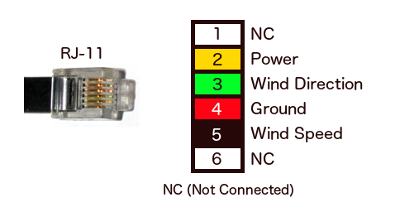
\includegraphics[width=0.5\textwidth]{img/rj11.png}
	\caption{Esquema conexionado RJ11}
	\label{fig:rj11}
\end{figure}
\newpage

\subsection{Dirección del viento}
Para obtener la dirección del viento es necesario conectar la salida del conector RJ11 con uno de los pines analógicos del Arduino. El sensor incorpora un potenciómetro de 20k$\Omega$ (figura \ref{fig:schema}) que conectaremos al conversor A/D del Arduino. El conversion tiene una resolución de 10bits, lo que nos da un rango de valores de 0 a 1023, que corresponde a su vez a un voltage de 0 a 5V. Mediante código (script \ref{app:script1}) debemos convertir el rango de valores del A/D al rango de 0 a 360º que ofrece el sensor para obtener la dirección del viento.

\begin{figure}[h]
	\center
	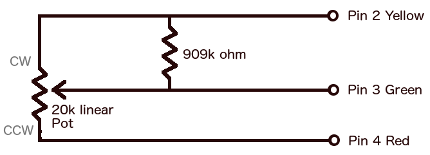
\includegraphics[width=0.65\textwidth]{img/schema.png}
	\caption{Esquema elétrico de la veleta}
	\label{fig:schema}
\end{figure}

El potenciómetro tiene una "banda muerta" que dará como resultado 0º en el rango 1020 - 4 como se puede apreciar en la figura \ref{fig:direction}. El sensor está calibrado de fábrica para entregar 0 cuando la dirección está alineada con el mástil que lo sostiene.

\begin{figure}[h]
	\center
	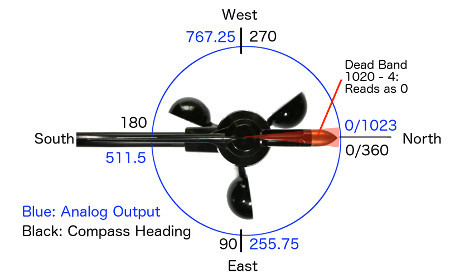
\includegraphics[width=0.65\textwidth]{img/direction.jpg}
	\caption{Esquema de la dirección}
	\label{fig:direction}
\end{figure}

\subsubsection{Resultados}
Para observar los resultados se ha optado en primera instancia por enviar los valores crudos obtenidos del sensor en una primera columna y los valores ya procesados por el conversor en una segunda columna a través del puerto analógico. Un script de Python (\ref{app:script4}) captura los valores del puerto serie y los almacena en un archivo de texto; posteriormente, un segundo script de Pyhton (\ref{app:script5}) los representa gráficamente. Los valores mostrados en la figura \ref{fig:testdirection1} se han obtenido girando la veleta de forma manual.

\begin{figure}[h]
	\center
	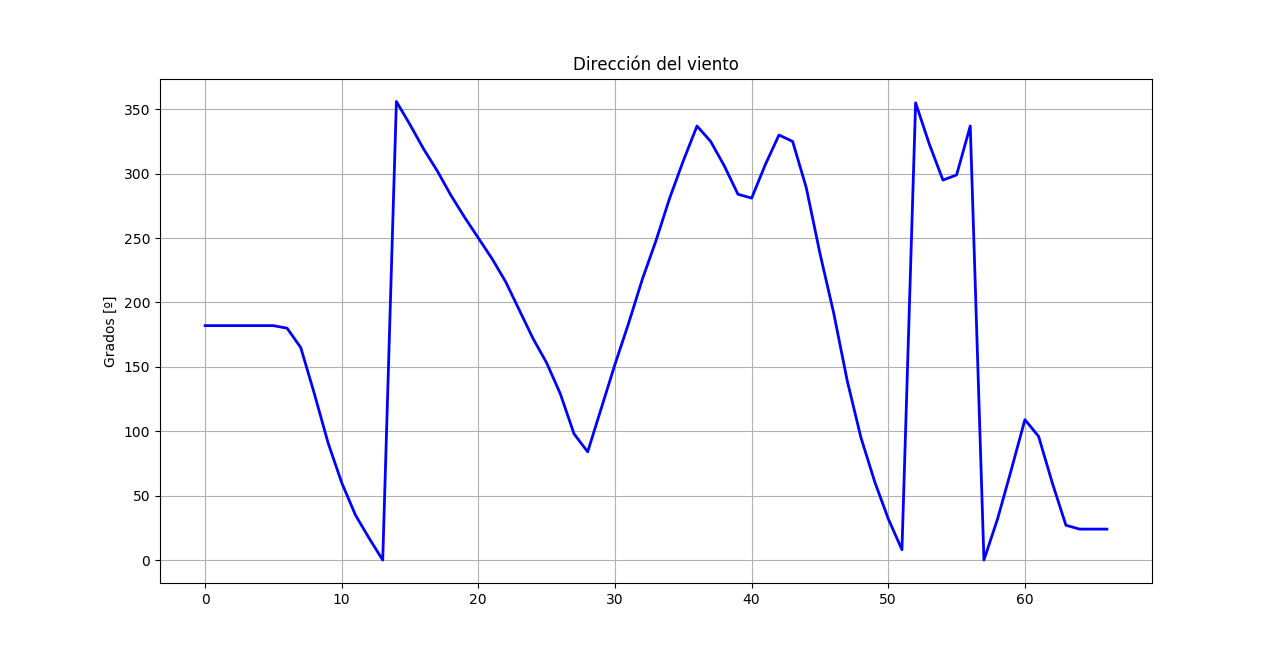
\includegraphics[width=1\textwidth]{img/testDirectionIn.png}
	\caption{Resultado de la primera prueba en interior}
	\label{fig:testdirection1}
\end{figure}

\subsubsection{Calibración del sensor}
La forma ideal de montage y funcionamiento del sensor es alinear la punta de la veleta con el mástil de sujeción. Aun así, si por condiciones físicas no es posible encarar el sensor con el norte magnético, debemos aplicar un \textit{offset} a nuestros cálculos para corregir la dirección del viento.

\begin{figure}[h]
	\center
	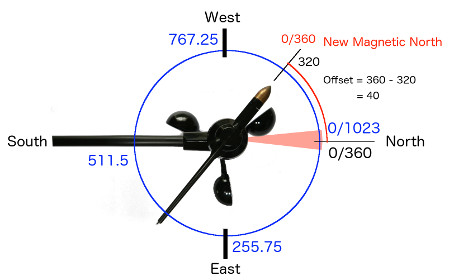
\includegraphics[width=0.65\textwidth]{img/offset.jpg}
	\caption{\textit{Offset} en la calibración de la dirección del viento}
	\label{fig:offset}
\end{figure}

Para determinar el valor de \textit{offset} que debemos aplicar, necesitamos apuntar la veleta hacía el norte magnético. Con la ayuda de una brújula vamos a determinar los grados de desviación, para luego restarlo al valor calculado.
\newpage

\subsection{Velocidad del viento}
Para obtener la dirección del viento es necesario conectar la salida negra del conector RJ11 con uno de los pines digitales del Arduino a través de un pull-up de 4k7$Omega$ que pondrá a 5V el pin del Arduino. 

Las copas para medir la velocidad del viento tienen un pequeño interruptor de lámina junto al eje de rotación, que se activa una vez cada rotación (figura \ref{fig:schema2}). Para calcular la velocidad del viento aplicaremos una fórmula que convierte el número de veces que se activa el interruptor por unidad de tiempo a km/h.

\begin{figure}[h]
	\center
	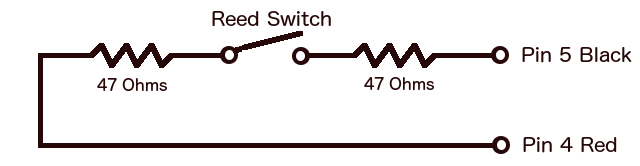
\includegraphics[width=0.65\textwidth]{img/schema2.png}
	\caption{Esquema elétrico anemómetro}
	\label{fig:schema2}
\end{figure}

De acuerdo con la documentación oficial de Davis, 1 milla por hora equivale a 1600 revoluciones por hora. Como vamos a trabajar a nivel europeo, la conversión se hará a quilómetros por hora, según la relación: 1 mph = 1,609344 km/h.

Usando la fórmula \ref{eq:formula} calcularemos la velocidad en km/h. Los parámetros que la definen son:

\begin{itemize}
	\item \textbf{V} $\rightarrow$ Velocidad en km/h.
	\item \textbf{P} $\rightarrow$ Número de pulsos por período.
	\item \textbf{T} $\rightarrow$ Período en segundos. 
\end{itemize}

\begin{equation} 
V = P \cdot \left(\frac{3.621024}{T}\right)
\label{eq:formula}
\end{equation}

A causa de activaciones naturales incontroladas del interruptor, se ha decidido trabajar con interrupciones en el pin digital del Arduino que generan una interrupción en el flanco descendente del pulso que incrementa un contador.

Se usa un \textit{delay} de 3 segundos para obtener una media de la dirección del tiempo; este valor es T en la fórmula de cálculo. 

\subsubsection{Resultados}
A diferencia de la primera parte, ahora no obtenemos unos datos en crudo, sino que se calcula según el número de rotaciones por período. Para observar los resultados se ha optado por guardar en una primera columna el número de rotaciones por período y en una segunda columna el valor de la velocidad. La figura \ref{fig:testvelocity1} representa la primera prueba, en la que se ha soplado el anemómetro en un espacio cerrado.

\begin{figure}[h]
	\center
	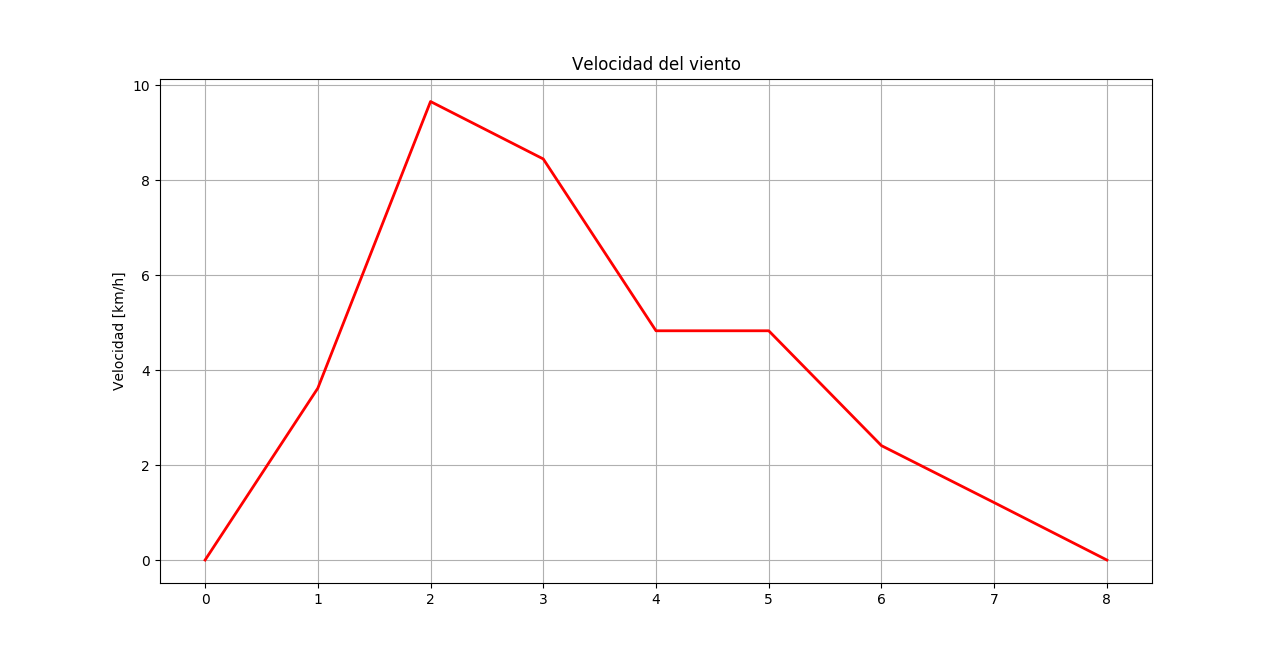
\includegraphics[width=1\textwidth]{img/testVelocityIn.png}
	\caption{Resultado de la primera prueba en interior}
	\label{fig:testvelocity1}
\end{figure}
\newpage

\section{Resultados finales}
Una vez comprobado el buen funcionamiento de los sensores de forma separada, es vital crear un script que capture los datos de los dos sensores para obtener los resultados a la vez (script \ref{app:script3}). 

El resultado se ha representado de forma gráfica  (figura \ref{fig:testfull}) mediante el script de Python previamente citado con la peculiaridad que se representa cada sensor en un eje Y distinto, pero compartiendo el mismo eje X; de esta forma es más visual la evolución de los datos.

\begin{figure}[h]
	\center
	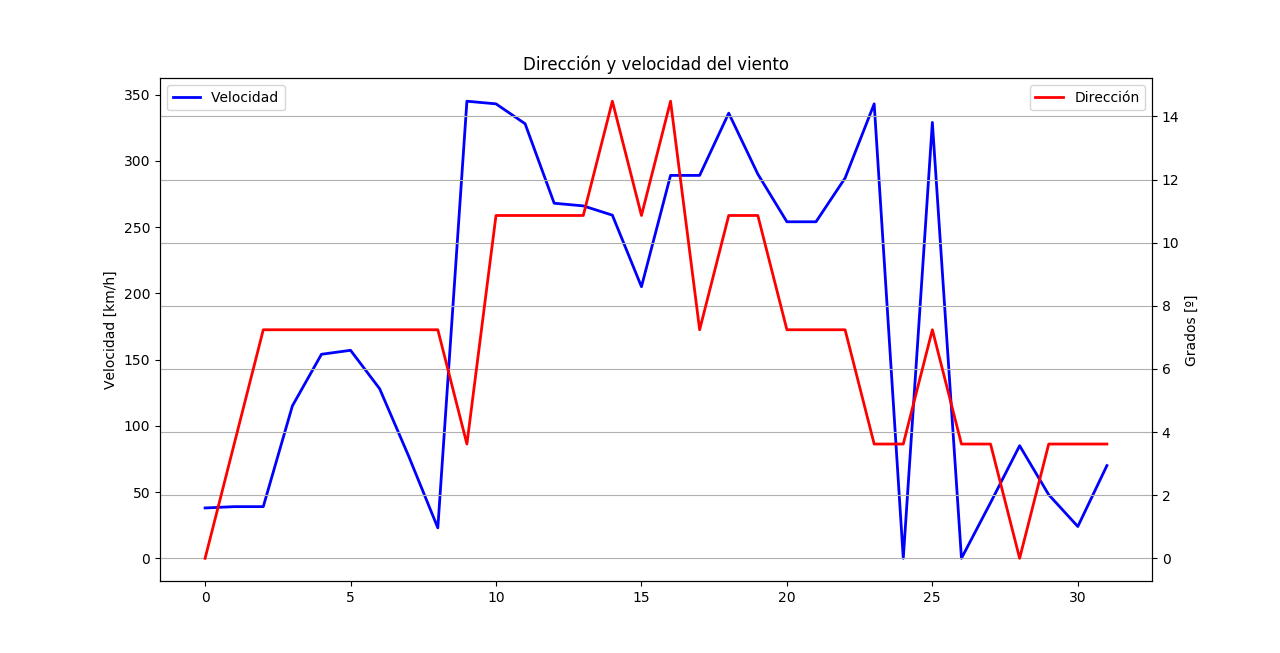
\includegraphics[width=1\textwidth]{img/testFullIn.png}
	\caption{Resultado conjunto en interior}
	\label{fig:testfull}
\end{figure}
\newpage

\begin{thebibliography}{9}
\addcontentsline{toc}{section}{References}
\bibitem{Arduino website}
Arduino: Python interfacing,
\\\url{https://playground.arduino.cc/Interfacing/Python}

\bibitem{Cactus website}
Cactus io,
\\\url{http://cactus.io/hookups/weather/anemometer/davis/hookup-arduino-to-davis-anemometer}

\bibitem{Davis website}
Davis Instruments,
\\\url{http://www.davisnet.com}

\bibitem{Python matplotlib}
Python: Matplotlib,
\\\url{https://matplotlib.org}
\end{thebibliography}
\newpage

\section*{Anexos}
\addcontentsline{toc}{section}{Anexos}
\appendix
\renewcommand{\thesection}{\Alph{section}}
Todo el código utilizado para el desarrollo del proyecto se puede encontrar en GitHub: \url{https://github.com/polrodoreda/CaptorProject}.

\section{Script windDirection.ino}
\label{app:script1}
\begin{lstlisting}[basicstyle=\small, language = C++]
int VaneValue;
int Direction;
int CalDirection;

#define Offset 0;

void setup() {
  Serial.begin(9600);
  Serial.println("Wind Direction");
  Serial.println("Vane Value \t Direction");
}

void loop() {
  VaneValue = analogRead(A4);
  Direction = map(VaneValue, 0, 1023, 0, 360);
  CalDirection = Direction + Offset;

  if (CalDirection > 360) 
    CalDirection = CalDirection - 360; 

  if (CalDirection < 0) 
    CalDirection = CalDirection + 360; 

  Serial.print(VaneValue);
  Serial.print("\t");
  Serial.println(CalDirection);
  
  delay(500);
}
\end{lstlisting}
\newpage

\section{Script windVelocity.ino}
\label{app:script2}
\begin{lstlisting}[basicstyle=\small, language = C++]
#include <math.h>

volatile unsigned long Rotations;
volatile unsigned long ContactBounceTime;

float WindSpeed;

void setup() {
  Serial.begin(9600);
  pinMode(2, INPUT);
  attachInterrupt(digitalPinToInterrupt(2), isr_rotation, FALLING);

  Serial.println("Wind Velocity");
  Serial.println("Rotacions \t km/h");
}

void loop() {
  Rotations = 0;

  sei();
  delay(1000);
  cli();

  WindSpeed = (3.621024/1) * Rotations;
  Serial.print(Rotations);
  Serial.print("\t");
  Serial.println(WindSpeed);
}

void isr_rotation() {
  if ((millis() - ContactBounceTime) > 15) {
    Rotations++;
    ContactBounceTime = millis();
  }
}
\end{lstlisting}
\newpage

\section{Script windFull.ino}
\label{app:script3}
\begin{lstlisting}[basicstyle=\small, language = C++]
#include <math.h>

volatile unsigned long Rotations;
volatile unsigned long ContactBounceTime;

float WindSpeed;
int VaneValue;
int Direction;
int CalDirection;

#define Offset 0;

void setup() {
  Serial.begin(9600);
  pinMode(2, INPUT);
  attachInterrupt(digitalPinToInterrupt(2), isr_rotation, FALLING);

  Serial.flush();
}

void loop() {
  //Direction
  VaneValue = analogRead(A4);
  Direction = map(VaneValue, 0, 1023, 0, 360);
  CalDirection = Direction + Offset;

  if (CalDirection > 360) 
    CalDirection = CalDirection - 360; 

  if (CalDirection < 0) 
    CalDirection = CalDirection + 360; 

  //Speed
  Rotations = 0;

  sei();
  delay(1000);
  cli();

  WindSpeed = (3.621024/1) * Rotations;
  
  Serial.print(CalDirection);
  Serial.print("\t");
  Serial.println(WindSpeed);
}

void isr_rotation() {
  if ((millis() - ContactBounceTime) > 15) {
    Rotations++;
    ContactBounceTime = millis();
  }
}
\end{lstlisting}
\newpage

\section{Script readSerial.py}
\label{app:script4}
\begin{lstlisting}[basicstyle=\small, language = Python]
#-*- encoding:utf-8 -*-
import sys
import serial

try:
    ser = serial.Serial('/dev/cu.usbmodem1411', 9600)
except:
    print 'Error de conexion'
    sys.exit()

data_file = sys.argv[1]
f = open(data_file, "w")

while True:
    try:
        f.write(ser.readline())
    except (KeyboardInterrupt):
        f.close()
        sys.exit()
\end{lstlisting}
\newpage

\section{Script plotData.py}
\label{app:script5}
\begin{lstlisting}[basicstyle=\small, language = Python]
#-*- encoding:utf-8 -*-
import sys
import matplotlib.pyplot as plt

def read_data(filename, t):
    f = open(filename, "r")
    data = []
    dataFull = [[], []]

    for line in f.readlines():
        if t == 'D' or t == 'V':
            data.append(line.split("\t")[1])
        else:
            dataFull[0].append(line.split("\t")[0])
            dataFull[1].append(line.split("\t")[1])

    if t == 'D' or t == 'V':
        return data
    else:
        return dataFull

def plot(data, t):
    if t == 'D':
        plt.plot(data, 'b', linewidth = 2)
        plt.title(u'Direccion del viento')
        plt.ylabel(u'Grados')
    elif t == 'V':
        plt.plot(data, 'r', linewidth = 2)
        plt.title(u'Velocidad del viento')
        plt.ylabel(u'Velocidad [km/h]')
    else:
        fig, ax1 = plt.subplots()
        ax1.plot(data[0], 'b', linewidth = 2, label = u'Velocidad')
        ax1.set_ylabel(u'Velocidad [km/h]')
        ax1.legend(loc = 2)

        ax2 = ax1.twinx()
        ax2.plot(data[1], 'r', linewidth = 2, label = u'Direccion')
        ax2.set_ylabel(u'Velocidad [km/h]')
        ax2.set_ylabel(u'Grados')
        ax2.legend(loc = 0)

        plt.title(u'Direccion y velocidad del viento')

    plt.grid(True)
    plt.show()

if __name__ == '__main__':
    filename = sys.argv[1]
    t = filename[4]
    data = read_data(filename, t)
    plot(data, t)
\end{lstlisting}
\end{document}